

\documentclass[11pt,a4paper,titlepage,oneside]{article}

\usepackage[most]{tcolorbox}
\usepackage{geometry}
\usepackage{svg}

\usepackage{hyperref} %links
\usepackage{xurl}

\usepackage[document]{ragged2e} %floating text
\usepackage{helvet} %font
\usepackage{tocloft} % dots in table of contents sections

\usepackage{lipsum, multicol}
\usepackage{fancyhdr}
\usepackage{listings}


% citaitons
\usepackage{natbib}

% hypthenationrules
\usepackage[T1]{fontenc}



%redefine the entire fucking bib environment so we dont have the horisontal spacing
% this was generated entirely by chatgpt

\makeatletter
\renewenvironment{thebibliography}[1]
  {\section{Lähteet}%
   \@mkboth{\MakeUppercase{\refname}}{\MakeUppercase{\refname}}%
   \list{\@biblabel{\@arabic\c@enumiv}}%
        {\settowidth\labelwidth{\@biblabel{#1}}%
         \leftmargin\labelwidth
         \advance\leftmargin\labelsep
         \setlength\itemindent{-\labelwidth}
         \setlength\itemsep{10pt} % Change this value to adjust the space between items
         \@openbib@code
         \usecounter{enumiv}%
         \let\p@enumiv\@empty
         \renewcommand\theenumiv{\@arabic\c@enumiv}}%
   \sloppy
   \clubpenalty4000
   \@clubpenalty \clubpenalty
   \widowpenalty4000%
   \sfcode`\.\@m}
  {\def\@noitemerr
    {\@latex@warning{Empty `thebibliography' environment}}%
   \endlist}
\makeatother





%this is such a shitshow lmao

\hypersetup{
    colorlinks=false,
    citecolor=black,
    filecolor=black,
    linkcolor=black,
    linkbordercolor=1 1 1,
    citebordercolor=1 1 1,
    pdfborderstyle={/S/U/W 1},
    urlbordercolor=0 0 1,
    urlcolor=blue
}
\urlstyle{same}



\geometry{
    a4paper,
    left=3cm,
    right=2.5cm,
    top=3cm,
    bottom=2.5cm
}

%remove random margin on side ? idk what happend
%\setlength{\oddsidemargin}{0pt}


%these need to be overridden in coverpage
\renewcommand{\baselinestretch}{1.5} 
\setlength{\parskip}{0.1cm}


%custom reusable colorbox rules
\newtcolorbox{simplebox}{colback=white, sharp corners, boxrule=1pt }


\renewcommand{\contentsname}{Sisällys} % override Contents => Sisallys on table of contents
\renewcommand{\cftsecpagefont}{\normalfont} %remove section bold font in toc
\renewcommand{\cftsecfont}{\normalfont}% remove section bold font in toc
\setlength{\cftbeforesecskip}{0px} % remove weird vfill between toc sections


\renewcommand{\familydefault}{\sfdefault} % set font

\renewcommand{\cftsecleader}{\cftdotfill{\cftdotsep}} % dots for sections

\renewcommand{\bibsection}{\section{Lähteet}} % bibbliio name on lähteet sectio

\setlength{\headheight}{13.6pt}


\def\filename{src/oppari.tex}



\def\testmode{1}






\newcommand\wordcount{
    \immediate\write18{texcount -sub=section \filename{} -inc  | grep Section | sed -e 's/+.*//' | sed -n \thesection p > 'count.txt'}
(\input{count.txt}words)}


\newcommand{\inputf}[1]{\def\filename{#1}\input{#1}}


\newcommand\filewcount{
    \immediate\write18{texcount -1 -sum \filename{} > count.txt }
    \input{count.txt} words }


% jos on testi definetty niin tee 
\newcommand{\istest}[2]{\ifx\testmode\undefined #2 \else #1 \fi}


% testi section näyttää word countin siltä sectionilta jos ei testi niin sitten näytä vain normaali section
\newcommand{\tsection}[2]{\istest{#1{#2\\} \wordcount \\ \medskip }{#1*{#2}}}


\newcommand{\pagesection}[1]{\istest{\section{#1}  }{\section*{#1}}}
\newcommand{\pagesubsection}[1]{\istest{\subsection{#1}  }{\subsection*{#1}}}


% adds page with everything
\newcommand{\addPage}[2]{
    \def\filename{#1}
    \pagesection{#2}
    \istest{ \filewcount \medskip }{}
    \input{#1}
}



% OPPARI SPESIFIC

\newcommand{\addPageOp}[2]{
    \def\filename{#1}
    \pagesubsection{#2}
    \istest{ \filewcount \medskip }{}
    \input{#1}
}

%lab citation style
\newcommand{\labcite}[1]{\setcitestyle{aysep={},open={(},close={.)}}\citep{#1}{}}

%lab citation style
\newcommand{\labciteend}[1]{\setcitestyle{aysep={},open={(},close={).}}\citep{#1}{}}

\newcommand{\labimgcite}[1]{\setcitestyle{aysep={},open={(},close={)}}\citep{#1}{}}

\newcommand{\hurl}[1]{\href{#1}{{\underline{\textcolor{blue}{#1}}}}}


% counter kuville
\newcounter{imgCounter}
\setcounter{imgCounter}{0}

\newcommand{\getImgCount}{
\addtocounter{imgCounter}{1}
\theimgCounter
}


% counter kaavioille
\newcounter{chartCounter}
\setcounter{chartCounter}{0}

\newcommand{\getChartCount}{
\addtocounter{chartCounter}{1}
\thechartCounter
}



\usepackage[finnish]{babel}




\iffalse

random shit that we need to do

change words

Client => asiakasohjelma
    jotenkin tuntuu oudolta sanoo frontendiä asiakasohjelmaksi
    vissii selainohjelma??

Server => palvelinohjelma




\fi










% ------------------------------ BEGIN DOCUMENT ------------------------------ %
\begin{document}

\pagestyle{empty}


%------------------------------ COVER PAGE ------------------------------ %


\includegraphics[width=5cm,height=1cm]{./src/labimg.jpg}

%override baselinestretch thing in this area
\renewcommand{\baselinestretch}{1} 
\setlength{\parskip}{0cm}

\vspace{86mm}
{\huge
\textbf{Kehityksen seuranta}
}
\newline

{\large

\vspace{5mm}
\textbf{Oppimispäiväkirja}
}

\vspace{90mm}

LAB-ammattikorkeakoulu \newline
\vspace{2mm}
Tieto-ja tietolikenadsfklj, Insinööri (AMK) \newline
\vspace{2mm}
2024 \newline
\vspace{2mm}
Kimi Malkamäki

\newpage

%reset thing
\renewcommand{\baselinestretch}{1.5} 
\setlength{\parskip}{0.1cm}



%------------------------------ FIRST PAGE OF ABSTRACT ------------------------------ %
\begin{tabular}{ | l | }

    %hack for the tiivistelmä line
    \multicolumn{1}{l}{
        \begin{minipage}{6cm}
            \hspace{1mm}
            
        \end{minipage}
        \begin{minipage}{4.25cm}
            \hspace{1mm}
        \end{minipage}
        \begin{minipage}[t][1.95cm][t]{3.62cm}
            \large
            \textbf{ Tiivistelmä }
        \end{minipage}
    }\\

    \hline
    \begin{minipage}[b]{6cm}
        tekijä(t)
        \newline
        kimi malkamäki 
    \end{minipage}%
    % 2x2
    \begin{minipage}{8.5cm}
        \begin{tabular}{ | l | c | }
            \begin{minipage}[t][1cm][t]{4.25cm}
                julkaisun laji
                \newline
                Opinnäytetyö, AMK
            \end{minipage} & %
            %
            \begin{minipage}{3.62cm}
                valmistusaika
                \newline
                2024
            \end{minipage} \\ \hline%
            %
            \begin{minipage}[t][1cm][t]{4.25cm}
                sivumäärä
                \newline 
                xx+xx
            \end{minipage}
            &  \\ \hline
        \end{tabular}
    \end{minipage}%
    % end of 2x2
      \\ \hline

    \begin{minipage}[t][2cm][t]{8cm}
    Työn nimi 
        \newline 
    ammatissa kasvaminen 
        \newline 
    oppimispäiväkirja  
    \end{minipage}\\ \hline

    \begin{minipage}[t][1.5cm][t]{10cm}
    tutkinto ja koulutusala.\newline  tietoviestintätekniikka insinööri amk  

    \end{minipage}\\ \hline

    \begin{minipage}[t][7cm][t]{5cm}
    tiivistelmä: \newline lorem ipsim
    \end{minipage}\\ \hline

    \begin{minipage}[t][2cm][t]{5cm}
    avain sanat
    \end{minipage}\\ \hline

\end{tabular}

\newpage



% ------------------------------ SECOND PAGE OF ABSTRACT ------------------------------ %

tiivistelmä








\newpage


% ------------------------------ TABLE OF CONTENTS ------------------------------ %


%keep page numbers off
\setcounter{page}{0}
\pagestyle{empty}
\pagenumbering{gobble}

\tableofcontents





\newpage



% ------------------------------- TERMISTÖ ------------------------------- %


TERMISTÖ
\bigskip

(tiedän ettei termistö kirjoiteta tällä formaatilla. tämäkin on hyvin kesken)
\bigskip
 
%this needs to be aligned cannot be like this make minipage maybe
ECMAscript = skriptaus-kieli standardi 
\bigskip

DOM = Document Object Model 
\bigskip

puu = datastruktuuri(selitä paremmin)
\bigskip

VDOM = virtual DOM
\bigskip

Transpilaatio = ohjelmointikielen kääntäminen toiseen ohjelmointikieleen
\bigskip

CSS = Cascading Style Sheets
\bigskip

client = asiakasohjelma
\bigskip


\newpage





% ------------------------------- CONTENT PRELUDE COMMANDS ------------------------------- %
%enable page counting
\pagenumbering{arabic}
\clearpage
\setcounter{page}{1}

%set heaader and footer
\pagestyle{fancy}
%%
\lfoot{}
\cfoot{}
\rfoot{}
%%
\lhead{}
\chead{}
\rhead{\thepage}
%%
\renewcommand{\headrulewidth}{0pt}
\renewcommand{\footrulewidth}{0pt}


%\newcommand{\n}{\newline\vspace{20mm}}





    






\section{Johdanto}              % ------------------------------- JOHDANTO ------------------------------- %


% vaatii uudelleen kirjoittelua 
% ainakin toinen kappale



Teknologia ala on nopeasti liikkuva, uusien teknologioiden kehittyessä vanhat teknologiat poistuvat käytöstä.
Alan-ammattilaisen pitää pysyä valppaana, ja aktiivisesti opiskella uusia teknologioita, 
että hän pystyisi pysymään ajantasalla nykyisistä alan suuntauksista.
Uudet työkalut ohjelmointikiele 
%needs more
\medskip



% ei mainita liitettä tässä. sanotaan vaan että on päiväkirja mainen ja että on seurantajakso 

%eli kokonaan alusta ja uusiks
Opinnäitetyö on kirjoitettu päiväkirja mallilla
ja ennen opinnäytettyön kirjoittamista suoritettiin 13 viikon seurantajakso, jolloin
kirjasin minkä teknologian kanssa työskentelin ja mitä tein ja opin viikon aikana.
% selitys siitä miksi tämä on hyvä ja miten se liittyy ylempääänn kappaleeseen
Päiväkirja antaa hyvän silmäyksen työskentelemisestä ohjelmistokehittäjänä tieto- viestintätekniikan alalla, 
ja haasteista mitkä ilmeentyvät päivittäin.% tähän voi lisätä vielä yhden jos keksii
%
% jotain lisää siitä että pvkirja antaa silmäyksen elämään itse ammattilaisena,
% jolla on juuri ongelmia mitkä kuvattiin  ekassa kappaleessa
%tässä voi olla joku concrete esimerkki siitä mitä tehtiin ja mitä tehdään
%
% mainitaanko että opin vai pitääkö johdannossa olla tulevaisuus presenssi
Seurantajakson aikana opin minulle uusista teknologioista ja web alustojen kehittämisestä.
\medskip



% tätä ennen tulee jotain tekstiä itse tavoite sanotaan tiivistelmässä vissiinkin
Opinnäytettyön tavoitteena on seurata kehitymistä ja teknologoiden oppimista seurantajakson aikana,
jolloin kirjoitettiin oppimispäiväkirja.
% kirjoitetaanko lisää itse pvkirjasta tähän?
Oppimispäiväkirja on kirjoitettu teemoittain teknologioista mitä käytin ja opiskelin seurantajakson aikana.
Teemat voivat kattaa useamman viikon ja niissä kerrotaan itse teknologiasta, miten käytin kyseistä teknologiaa viikon tehtävien toteuttamiseen ja
ongelmiin joihin törmäsin niitä käyttäen.
%more text
\medskip




%selitys starttaamosta ja mistä se tekee/haluaa

Opinnäytetyö toteutettiin Starttaamo Oy:ssä. Starttaamo on suomalainen startup yritys, joka pyrkii ratkomaan ongelmia työergonomian kanssa.
Startupin pää tavoitteena on vähentää sairaslomia saamalla työntekijät noudattamaan, alojen ammattilaisten suunnittelemien liikunta- ja ruokavalio-ohjelmia. 
% scuffed af.. web alusta jota kehitin...  jotenkin paremmin se että olin kehittämässä sitä mukana.
Yrityksen pää myyntituote on web-alusta, jonka kehityksen mukana olin.
%
Alustan kehittämisessä sain mahdollisuuden työskennellä tuotantoympäristössä ja minulle uusien teknologioiden kanssa.
Olin mukana suunnittelussa, ominaisuuksien lisäämisessä ja ohjelmoinnissa. 
Sain myös kokemusta ilmeentyvien ongelmien korjaamisesta.

%more
\medskip










\newpage
\section{Lähtötilanne}         % ------------------------------- LÄHTÖTILANNE ------------------------------- %
% Tämä on suurimmaksi osaksi fine
% johannalta pitää kysyä kauan on ollut käynnissä ennen kun tulin ja kauan suunnittelussa
% mahdollisesti sanan vaihto frontend ja backend




Ennen opinnäytetyön kirjoittamista ja seurantajakson alkamista olin opiskellut LAB ammattikorkeakoulussa 7 lukukautta ja
olin opinnäytetyön kirjoituksen aikana neljännen vuoden tieto- ja viestintätekniikan opiskelija.
Vaikka minulla ei ollut aiempaa työkokemusta tieto- ja viestintätekniikan alalta ennen harjoituksen alkamista,
olin koulutuksen aikana saanut laajan pohjan ohjelmoinnista,
sen perusteista ja muista tieto- ja viestintätekniikan alan taidoista esim. versionhallinnasta, tietokannoista sekä web suunnittelusta.
Teoriapohja ei kuitenkaan aina riitä työelämässä, joten uusiin olosuhteisiin soveltuminen ja uusien asioiden oppiminen on oleellista.
\medskip



Harjoituksen aikana halusin oppia web alustojen kanssa työskentelystä ja projektissa käytetyistä teknologioista.
Halusin myös kokemusta työskennellä isommassa koodipohjassa, jota muutkin henkilöt ovat olleet suunnittelemassa.
Isommat projektit vaativat palavereita ja yhteenvetoja, että kaikki kehittäjät pysyvät ajan tasalla.
Sosiaaliset taidot ja kyky selittää teknisiä asioita asiakielellä on myös taito, 
jota en ollut ennen harjoittelua tarvinnut, mutta huomasin sen olevan oleellinen osa työelämää.
Viikoittaisten palavereihin osallistuminen ja viikon aikana tehtyjen töiden esittely ja selittäminen on oleellinen osa isommassa projektissa työskentelemistä.
\medskip

% front back en tiedä jos suomenkielinen olisi hyvä

Web sovelluksen kehittämisessä tulee esiin haasteita, joita ei tule muussa sovelluskehityksessä.
Sovellukset koostuvat useimmiten monesta osasta, kuten front-end, back-end ja tietokanta.
Nämä osat pitää olla jatkuvasti toiminnassa ja yhteyksissä toisiinsa sovelluksien toimimiseen ja niiden katkeaminen voi
johtaa sovelluksen toimimattomuuteen.
Myös palvelin- tai muut sovellus virheet voivat kaataa koko sovelluksen kaikille käyttäjille. 
Web sovelluksien kehittämisessä on myös etuja tavalliseen sovelluskehitykseen verrattuna, kuten 
web sovelluksen päivityksen saanti käyttäjille on nopeaa ja kaikki käyttäjät saavat päivityksen samanaikaisesti.
\medskip

Harjoituksen aika työskentelin Startupin web alustan kanssa. 
Olin mukana sen kehityksessä, suunnittelussa, ominaisuuksien lisäämisessä ja sivustojen ylläpidossa.
Alusta oli käyttöönotettu ennen harjoituksen alkamista ja siellä oli aktiivisia käyttäjiä.
Alusta on ollut käytössä X vuotta ennen harjoituksen alkamista ja sitä ennen X vuotta suunnittelussa.
Alustan kehityksessä, oli tehostettu kehitysnopeuteen,
joten alustalta puuttui monia ominaisuuksia, joita odotetaan web sovelluksesta, 
kuten web sivustojen kääntäminen ja sivustojen toimiminen mobiililaitteilla.
\medskip

























\newpage
\section{Teoria}                % ------------------------------- TEORIA ------------------------------- %



\subsection{Kehitys ympäristö / Teknologia pino}
% tä on suurimmaks osaks hyvä ehkä pitää selittää markkinoilla pärjääminen en tiedä




% vähän paremmin selitys markkinoille pääsemisenn
Startup- ja muut kasvuyritykset hakevat nopeaa ja ketterää kehitystä markkinoilla pärjäämiseen.
Kehityksen nopeus voi myös riippua teknologioista, sillä jollain teknologioilla on helpompi ja nopeampi toteuttaa joitain ominaisuuksia.
Tämä pitää ottaa huomioon, kun valitaan mitä teknologioita käytetään sovelluksessa.
Pohjalla käytettyjen teknologioiden vaihtaminen on erittäin työlästä jälkikäteen,
joten päätös käytetyistä teknologioista tulee vaikuttamaan yhtiön kehityksen nopeuden.
Hidas sovelluskehitys voi haitata itse yrityksen mahdollisuuksia selvitä markkinoilla.
\medskip



Projektin teknologia pino pohjautuu MeteorJs kehykseen, joka on suunniteltu nopeaan kehittämiseen ja käyttöönottoon.
% tosi huono selitys meteorista
Meteor helpottaa kommunikointia käyttöliittymän, palvelimen ja tietokannan kanssa, 
mutta silti antaen vapauden valita muut käytettävät teknologiat, eikä lukitse käyttämään valmiiksi valittuja teknologioita.
Meteor ei määritä käytettyä käyttöliittymä kirjastoa mutta se silti tukee monia suosituimpia kehyksiä ja antaa helpon integraation niihin.
Projektiin on valittu ReactJs kirjasto käyttöliittymän toteutukseen.
Reactin komponentti pohjainen rakenne tekee käyttöliittymä koodista helposti uudelleen käytettävän, nopeuttaen käyttöliittymän rakentamista. 
Myös sen sisään rakennettu reaktiivisuus tilallisilla komponenteilla tuo helpon käyttöliittymä päivityksen.
Meteor integroituu React kirjaston kanssa suoraan laatikosta.
Tämä on nähtävillä, kun Meteor pystyy päivittää React komponentteja automaattisesti esimerkiksi Tietokantamuutoksien tapahduttua. 
Projektissa käytössä oleva tietokanta MongoDB on myös hyvin integroitu Meteoriin.
MongoDBn skeematon dokumentti rakenne, tuo helpon tavan päivittää skeemoja tarpeiden tullen.
\medskip


MeteorJs, MongoDB ja ReactJs on alustan pohjalla käytetyt teknologiat, jonka päälle projekti on rakennettu.
Yhdessä näitä kolmea teknologiaa käyttäen voi luoda monenlaisia nopeita ja skaalautuvia nettisivuja ja sovelluksia pienistä projekteista suuriin.
Nämä teknologiat ovat myös suunniteltu nopeaan kehittämiseen, joka tekee niistä hyvän valinnan kasvavalle startup yritykselle.
\medskip









\newpage
\addPageOp{src/op/meteor.tex}{Meteor}                % ------------------------------- Meteor ------------------------------- %




\newpage
\addPageOp{./src/op/react.tex}{React}% ------------------------------- REACT ------------------------------- %






\newpage
\addPageOp{./src/op/mongo.tex}{MongoDB}        % ------------------------------- MONGODB ------------------------------- %













\newpage
\subsection{Responsiiviset käyttöliittymät}        % ------------------------------- Responsive ------------------------------- %

% css media query osuus vaatii isompaa uudelleen kirjoittelua
% asettelu vaihtoehdot eka kappale vaatii lisää tekstiä


% layout => asettelu

\subsubsection{Responsiivisten käyttöliittymien suunnittelun periaatteet}

% ekassa kappaleessa on jotenkin outoo selitystä siitä että eri laitteita on olemassa



% selitä enemmillä sanoilla ja paremmin eri laitteiden käyttö
Tekniikan parantuessa verkkolaitteiden määrä on kasvanut, ja ihmiset käyttävät enemmän ja enemmän mobiili laitteita verkkosivujen selaamiseen \labcite{statista23b}
Kehittäjien pitää ottaa huomioon eri laitteiden muuttujat kuten, näytönkoot, kuvasuhde ja näytön resoluutio.
Uusien verkkosivujen luominen mobiili selaimille ei ole aina käytännöllistä, sillä niitä pitäisi ylläpitää erikseen työpöytäsivuista.
Saman verkkosivun käytön toiminta useammalla eri laitteella vaatii eri lähestymistapaa verkkosuunnitteluun. 
Sivuston asettelu pitää pystyä muuttumaan sopivaksi laitteelle.
Verkkosivujen suunnittelussa tätä lähestymistapaa kutsutaan responsiiviseksi suunnitteluksi. \labciteend{marcotte10}
\medskip



Responsiivinen verkkosuunnittelu on lähestymistapa verkkosivustojen rakentamiseen,
jolla varmistetaan niiden optimaalinen ulkoasu ja toimivuus eri laitteilla näytön koosta huolimatta. 
Responsiiviset verkkosivut mukautuvat käyttölaitteeseen, siten että ne voisi tarjota yhdenmukaisen käyttökokemuksen käyttölaitteesta riippumatta.\labcite{mozilla24a}
\medskip





\subsubsection{CSS Media query}


% eka kappale ei selitä kunnolla mikä on media query imo
% toinen kappale jos näytönkoko on pienempi kuin x on huono ja ko
%   vissii toinen kappale kokonaan uusiks








CSS (eng Cascading Style Sheets) antaa työkaluja millä kehittäjä voi tietää käytetystä laitteesta.
Näitä kutsutaan Media queryiksi.
Mediaqueryt mahdollistaa selain tai käyttölaite arvojen kyselyn ja testailun, ja mahdollistaa ehdollisen CSS tyylien asettelun.\labcite{mozilla24b}

\medskip




%yritä kirjoittaa tää tohon ylempään 

CSS Media Query antaa mahdollisuuden CSS-säännöksen asettamiselle vain silloin kun selain- ja laiteympäristö vastaa määritettyjä sääntöjä. 
Media Queryt ovat tärkeä osa repsonsiivista suunnittelua ja se antaa mahdollisuuden luoda erilaisia asetteluja riippuen käyttölaitteesta,
sen näytön koosta tai kuvasuhteesta.\labcite{mozilla24b}



%esimerkkejä mediaqueryista tai jotain vastaavaa









\subsubsection{Asettelu vaihtoehdot}

% eka kappale liian vähän tekstiä ja pitäis selittää juttuja paremmin



%fine?

sivujen elementtien asettelu ja niiden käytäntö eri olosuhteissa on tärkeä osa responsiivista suunnittelua.
Kolme suosittua asettelu vaihtoehtoa on fixed, fluid ja adaptiivinen\labciteend{ksenia23}
Nämä vaihtoehdot (selittävät) miten elementit toimivat eri käyttöolosuhteissa kuten mobiili laitteilla.
\medskip



Kiinteä asettelussa elementit pysyvät samana näyttökoosta huolimatta. 
Kiinteässä asettelussa tulee ongelmia, jos näytön koko on pienempi, kun sivustolle suunniteltu asettelu, 
sillä joitain elementtejä jäisi näytöstä ulkopuolelle tai saatavissa sivu skrollaamisella.\labcite{ksenia23}
\medskip


Nestemäisessä asettelussa elementtien koot vaihtuvat näytön koon mukaan. 
Verrattuna kiinteään asetteluun elementit eivät jää näytöstä ulkopuolelle sillä elementit skaalautuvat näytönkoon mukaan.
%selitä vähän paremmin
Nestemäisessä asettelussa tulee silti ongelmia sillä, jos elementti on liian pieni sille annetulle tekstille.\labcite{ksenia23}
\medskip


Adaptiivisessä asettelussa elementtien koot ja sijainnit muuttuvat riippuen näytönkoosta.\labcite{ksenia23}
Adaptiivisen asettelun ideana on mukauttaa sivuston elementtien asettelu sopivaksi käytetylle laitteelle.
Kuvassa \nextImageCount {} on esimerkki sivuston asettelusta, kuvassa {\the\numexpr \theimgCounter + 2 } on esimerkki miltä sivusto voisi näyttää, jos käytössä olisi adaptiivinen asettelu.
Käyttöliittymän elementit ovat siirtyneet vierekkäisestä asettelusta päällekkäiseen sopimaan pienempään näytönkokoon.
%more
\medskip


\bigskip
%kuvat medium artikkelin giffistä

\includegraphics[width = 15cm]{src/public/oppar/adaptiveBig.png}\\
Kuva \getImgCount {}. esimerkki adaptiivisesta asettelusta isommalla näytöllä \labimgcite{ksenia23}
 
\bigskip


\includegraphics[width = 15cm]{src/public/oppar/adaptivesmall.png}\\
Kuva \getImgCount {}. esimerkki adaptiivisesta asettelusta pienemmällä näytöllä\labimgcite{ksenia23}




















\newpage
\subsection{Web sivustojen kääntäminen}




%link tree
% https://www.linkedin.com/pulse/website-translation-how-to-guide-louise-souter


\subsubsection{motivaatio verkkosivustojen kääntämiseen}

%miksi kääntää sivustot------------------------------------


%väärä sitaatti


% people prefer content in their lenguage
%https://csa-research.com/Featured-Content/For-Global-Enterprises/Global-Growth/CRWB-Series/CRWB-B2C#10Facts
% 11.6


%https://localizejs.com/articles/convince-stakeholders-localization-roi-data
% roi on localisation. this could be cited in the first thing
% 27.6 



Kielimuuri on merkittävä haaste, kun tuotteita ja verkkosivustoja laajennetaan uusille markkinoille.
65\% verkkokäyttäjistä suosii sisällön esittämistä omalla äidinkielellään \labciteend{csa20}
Sisällön tarjoaminen useilla kielellä on loistava tapa kasvaa eri markkinoille. 
Kun ihmiset voivat lukea sivustoasi omalla äidinkielellään, heillä on todennäköisemmin miellyttävä käyttökokemus.
Tutkimukset myös osoittavat, että tuotteiden lokalisointi on hyvä sijoitus kohde.\labcite{austin18}
\medskip



Käyttäjien suosimus omakieliselle sisällölle korostaa tarkkojen käännösten tarjoamisen ratkaisevaa merkitystä.
Jos käännökset laiminlyödään, huomattava osa potentiaalisista käyttäjistä ei välttämättä pysty käyttämään tuotetta tehokkaasti.
Näin ollen yritykset ovat vaarassa vieraannuttaa suuren osan mahdollisista käyttäjistä.
% 
Siksi laadukkaisiin käännöksiin ja lokalisointeihin investoiminen on olennaisen tärkeää yrityksille,
jotka pyrkivät saavuttamaan maailmanlaajuista menestystä ja maksimoimaan tavoittavuutensa erilaisilla kielimarkkinoilla.
\medskip % tarvitseekö tämä sitaatiota...









\subsubsection{Käännös tavat ja haasteet}


%https://www.transifex.com/blog/2024/website-translation-methods/
%11.6 


% sitaatti sille että eri kielissä on eri kontextia eri sanoille jne
%jos nykyinen on huono käytä tätä
%https://www.smartling.com/resources/101/context-better-translations/

% sitaatti ai käännös vs ihmis käännös


On useita eri tapoja web sivustojen kääntämiselle.
Mutta, koska monet kielet ovat hyvin erilaisia konteksti ja nyanssit voivat hävitä, jos käännetään sana sanaan.
Monia lauseita ja ilmaisuja ei voi kääntää suoraan kielestä toiseen menettämättä niiden alkuperäistä merkitystä.
Esimerkiksi idiomit, metaforat ja puhekieliset ilmaisut edellyttävät usein luovaa mukauttamista eikä niinkään kirjaimellista kääntämistä. 
Lisäksi tietyt termit ja käsitteet voivat olla olemassa yhdessä kulttuurissa, 
mutta eivät toisessa, jolloin tarvitaan harkittuja selityksiä tai korvauksia, jotta sama viesti voidaan välittää tehokkaasti.\labcite{interpservices22}
\medskip



Käännös tekstin luonnin voi yleisesti tehdä kahdella tavalla. henkilökäännös tai tekoälykäännös.
Henkilökäännöksellä voi olla hyvä tarkkuus ja lopputulos tulee kuulostamaan luonnolliselta.
Tämä ratkaisu tulee olemaan kalliimpi tekoälykäännökseen verrattuna sillä oikea kääntäjä pitää palkata.
tekoäly käännös on nopea ja halpa, mutta ei vielä ole tarpeeksi tarkka kaikkiin käyttötarkoituksiin.\labcite{Habash23}
\medskip









% miten käännökset tehdään nettisivuille teknisesti ------------------------------------
% jotain vaihtoehtoja ja eri tapoja tehdä käännöksiä
\subsubsection{Käännökset teknisesti}

% eka kappale pitää uudelleen kirjoittaa
% toinenkin kappale pitää siirtää


% vaihda sanan valinta siihen että joskus ollaan tehty uusia kopioita joka käännetylle sivulle
% pitää vain uudelleen kirjoittaa

%sitaatti on olemassa siihen että on kopioitu joskus
%

% jos ei löydy mitään tähän niin on mahdollisuuis että pitää uudelleen kirjoittaa koko käänn sectio
% ellei sitä poisteta



%https://www.motionpoint.com/platform/what-are-the-best-technologies-for-website-translation/
% 11.6

%idk this sorce is so scuffed imo
%https://travod.com/blog/5-methods-translate-website
% 26.6
% tuossa on jotain mainintaa siitä että verkkosivun kopioinnista on oikea tapa 
% how can i not find a better src that mentions that this is used



Kopio verkkosivusta jossa sisältö on käännettynä, on vaihtoehto, joka ei vaadi erikoista teknologiaa itse sisällön kääntöä lukuunottamatta.
Tällä tavalla jokainen erikielinen sivusto voidaan muokata sopimaan juuri siihen kulttuuriin mihin se on kohdistettu.
Mutta monen eri version samasta verkkosivusta ylläpitäminen on työlästä, sillä muutoksien tekeminen pitäisi päivittää joka kopioon erikseen.
\medskip



% etsi joku src tähän. ei pitäisi olla vaikeaa



% more text or rewrite

Tekstin dynaaminen kääntäminen on toinen ja vähemmän työläämpi tapa kääntää verkkosivustoja.
Dynaamisessa kääntämisessä sivuston sisältö kääntyy paikallaan toiseen, riippuen käyttäjän valitusta kielestä.
Käännökset ja niiden tarkoitus on tallennettuna käännöstiedostoon, 
josta käyttöliittymä etsii halutut käännökset.\citemissing
Uuden testin lisääminen vaatii vain käännöksien lisäämisen käännöstiedostoon.
Tällä tavalla on helpompi lisätä uutta sisältöä, mutta eri kielisiä sivustoja ei voi mukauttaa.
\medskip

































\newpage
% mahdollissesti toteutus title pois että saa yhden lisää subsectiionin muuten tää on vähän liikaa alalukuja



% mahdollissesti toinen sectio missä puhun starttaamolla työskentelystä



\section{Käännösten toteutus}


% vaihda wip title title
% käyttöliitymä kohtaan tarvii pari tai yksi lause lisää 


\subsection{wip title tehtävä}


Starttaamo on hakenut nopeaa kehitystä web alustalle, joten kehityksen alkuvaiheessa 
ei olla huomioitu mahdollista tarvetta käännöksille. 
Tämä tarkoittaa sitä, että kaikki sivuston tekstit ovat kovakoodattu suomeksi.
Sivustojen julkisesti näkyvällä tekstillä ei ollut keskitettyä arkistoa vaan tekstit olivat sijoitettu komponentteihin.
\medskip

Sain työnaiheeksi rakentaa käännös järjestelmä, jonka avulla sivustot voitaisiin kääntää useammalle kielelle.
Käännös järjestelmmän pitäisi olla laajennettavissa siten että sivustojen päivittäminen ja uusien kielien lisääminen olisi 
olisi mahdollisimman nopeaa ja helppoa.\\
\medskip

Keskitetty arkisto missä kaikki sivuston julkinen teksti auttaisi käännösten tekemistä tulevaisuudessa,
sillä uusien kielien lisääminen ei vaatisi käyttöliittymä koodin muokkaamista.
Tekstin etsiminen koodipohjasta ei ollut monimutkaista nykyisien tekstimuokkaustyökalujen haku ominaisuuksilla.







\subsection{Käytetty teknologia}

% vaatii tekemistä
% eka kappale on kokonaan wip tekstiä
% kuviin pitää referoida ennen niitä joten tekstin sijaintia pitää siirtää
% muuten fine ehkä

% pitää testata
% kuulostaako tuo yksi kappale järkevältä


% uusiks melkein kokonaan

Meteorin kanssa yhteensopiva i18n kirjastoa käyttäen käännöksien luonti ei ole monimutkaista.
Kirjasto hakee käännökset käännöstiedostosta käännös funktion avulla.
Kuvassa \nextImageCount{} on esimerkki käännös funktiosta.
Kuvassa luodaan HTML paragraafi elementti, jossa kutsutaan käännösfunktiota. 
funktio hakee käännöstiedoston progress sivulta progress arvon.\\
\medskip

\bigskip
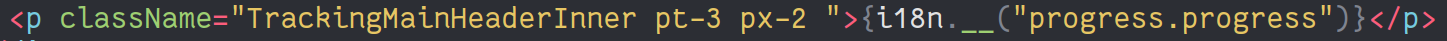
\includegraphics[width = 15cm]{src/public/oppar/translationcall.png}\\
Kuva \getImgCount. {} i18n käännösfunktiokutsu (ehkä uusi kuva)
\medskip


% emt onko incoherent

I18n kirjasto tukee montaa käännöstiedosto formaattia mutta päätin kirjoittaa ne JSON muotoon.
Kuvassa \nextImageCount{} on progressio sivun suomenkieliset käännökset ja kuvassa {\the\numexpr \theimgCounter + 2 } on saman sivun englannin kieliset käännökset.
Jokaisella sovelluksen sivulla on oma objekti, joka sisältää sen sivun julkisen tekstin. 
% en tiedä onko järkevän kuuloista
Avaimet tekstille on valmiiksi päätetyt muuttuja nimet, jotka kuvaavat käännöksen tarkoitusta.
Kun käyttäjä vaihtaa halutun kielen i18n osoittaa toiseen käännös tiedostoon, 
jossa on samat avaimet käännöksille mutta arvot ovat vaihtuneet kyseisen kielen käännöksiin.
\medskip


\bigskip
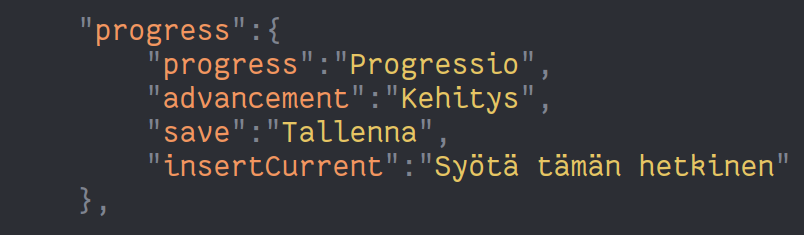
\includegraphics[width = 15cm]{src/public/oppar/translationfile.png}\\
Kuva \getImgCount. {} Progressiosivun suomenkielinen käännöstiedosto 
\medskip


\bigskip
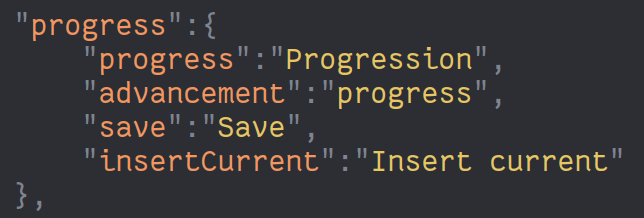
\includegraphics[width = 15cm]{src/public/oppar/translationfileEng.png}\\
Kuva \getImgCount {}. Progressiosivun englanninkielinen käännöstiedostosta
\medskip




\subsection{käyttöliittymä kielenvaihamiselle}

%lisäsin sivulle, tosin kun sivulle on lisätty

Sovellukseen on myös lisätty kuvan \nextImageCount{} laskuvalikko kielen vaihtamiselle. 
Kielet kuvataan lippuina laskuvalikossa,
sillä ne toimivat nopeina visuaalisina vihjeinä, jotka auttavat käyttäjiä tunnistamaan haluamansa kielen.
Laskuvalikko on näkyvissä sovelluksen kaikilla sivuilla, joten se on aina saatavilla.
\medskip



Laskuvalikon komponentti päivittää sovelluksen korkeamman React root komponentin kun käyttäjä on vaihtanut kielen.
Tällöin varmistetaan että kaikki sivuilla oleva teksti vaihtuu oikeaan kieleen.
%jotain pikkusen lisää
\medskip


\bigskip

\includegraphics[]{src/public/locale_laskuvalikko.png}\\
Kuva \getImgCount {}. Kielen vaihto laskuvalikko













\newpage
\addPage{src/op/feature.tex}{Uuden ominaisuuden lisäys} % ------------------------------- FEATURE ------------------------------- %










\newpage
\section{Yhteenveto}             % ------------------------------- YHTEENVETO ------------------------------- %

sehän meni ihan hyvin... 
lorem ipsum

opin käyttämään projektissa käytettyjä teknologioita
opin tekemään töitä ammatillisessa työympäristössä
\medskip


lokalisaatio meni hyvin ja sovellus on nyt parempi
\medskip


uusi ominaisuus toimii ja siitä ei tullut ognemlia sen käyttöönotossa
\medskip

\lipsum[1]




\newpage

% we need some way to manually override an item when it looks like shit

% i thin we need to make our own @ thing then use that for htings that look like shit
% though i dont thik we need the hfill thing in the first place but whattever that is problem for another day


(korjaa outo spacing)
\bibliographystyle{labCitations} % ------------------------------- LÄHTEET ------------------------------- %
\bibliography{./src/op/citations}


%https://libguides.eur.nl/overleaf/bibliographies-and-citing
%https://tex.stackexchange.com/questions/51434/biblatex-citation-order
% i want to do citations like this but if there is problem with the format then must do manually or... write own system





\section{Liitteet}               % ------------------------------- Liitteet ------------------------------- %

miten laitan liitteen päiväkirjasta ja millainen se pitäisi olla








\end{document}
